\documentclass{article}

\usepackage{ctex}
\usepackage{fancyhdr}
\usepackage{extramarks}
\usepackage{amsmath}
\usepackage{amsthm}
\usepackage{amssymb} 
\usepackage{amsfonts}
\usepackage{tikz}
\usepackage{url}
\usepackage{float}


%\usetikzlibrary{automata,positioning}

%
% Basic Document Settings
%

\topmargin=-0.45in
\evensidemargin=0in
\oddsidemargin=0in
\textwidth=6.5in
\textheight=9.0in
\headsep=0.25in


\pagestyle{fancy}
\lhead{\hmwkAuthorName}
\chead{\hmwkClass\ (\hmwkClassInstructor): \hmwkTitle}
\rhead{\schoolID}
\lfoot{}
\cfoot{\thepage}

\renewcommand\headrulewidth{0.4pt}
\renewcommand\footrulewidth{0.4pt}

\setlength\parindent{0pt}

%
% Create Problem Sections
%

\newcommand{\enterProblemHeader}[1]{
    \nobreak\extramarks{}{Problem \arabic{#1} continued on next page\ldots}\nobreak{}
    \nobreak\extramarks{Problem \arabic{#1} (continued)}{Problem \arabic{#1} continued on next page\ldots}\nobreak{}
}

\newcommand{\exitProblemHeader}[1]{
    \nobreak\extramarks{Problem \arabic{#1} (continued)}{Problem \arabic{#1} continued on next page\ldots}\nobreak{}
    \stepcounter{#1}
    \nobreak\extramarks{Problem \arabic{#1}}{}\nobreak{}
}

\setcounter{secnumdepth}{0}
\newcounter{partCounter}
\newcounter{homeworkProblemCounter}
\setcounter{homeworkProblemCounter}{1}
\nobreak\extramarks{Problem \arabic{homeworkProblemCounter}}{}\nobreak{}

%
% Homework Problem Environment
%
% This environment takes an optional argument. When given, it will adjust the
% problem counter. This is useful for when the problems given for your
% assignment aren't sequential. See the last 3 problems of this template for an
% example.
%
\newenvironment{homeworkProblem}[1][-1]{
    \ifnum#1>0
        \setcounter{homeworkProblemCounter}{#1}
    \fi
    \section{Problem \arabic{homeworkProblemCounter}}
    \setcounter{partCounter}{1}
    \enterProblemHeader{homeworkProblemCounter}
}{
    \exitProblemHeader{homeworkProblemCounter}
}

%
% Homework Details
%   - Title
%   - Due date
%   - Class
%   - Section/Time
%   - Instructor
%   - Author
%

\newcommand{\hmwkTitle}{Homework\ \#5}
\newcommand{\hmwkClass}{Pattern Recognition}
\newcommand{\hmwkClassInstructor}{Professor Wang Guijin}
\newcommand{\hmwkAuthorName}{{Qingyun~Fang} }
\newcommand{\schoolID}{{2017311003}}

\newcommand{\hs}{\hspace{2em}}
\newcommand{\vs}{\vspace{2ex}}
%
% Title Page
%

\title{
    \vspace{2in}
    \textmd{\textbf{\hmwkClass:\ \hmwkTitle}}\\
    %\normalsize\vspace{0.1in}\small{Due\ on\ \hmwkDueDate\ at 3:10pm}\\
    \vspace{0.5cm}\LARGE{\textit{\hmwkClassInstructor}}
    \vspace{4in}
}

\author{\hmwkAuthorName\\
{\schoolID}\\
Use \LaTeX ~in 4.18~2018} 


\date{}

\renewcommand{\part}[1]{\textbf{ Part \Alph{partCounter}}\stepcounter{partCounter}}

%
% Various Helper Commands
%


% Alias for the Solution section header
\newcommand{\solution}{\textbf{\Large Solution}}

% Probability commands: Expectation, Variance, Covariance, Bias
\newcommand{\E}{\mathrm{E}}
\newcommand{\Var}{\mathrm{Var}}
\newcommand{\Cov}{\mathrm{Cov}}
\newcommand{\Bias}{\mathrm{Bias}}

\linespread{1.5}

\begin{document}

\maketitle
\setcounter{page}{0}
\thispagestyle{empty}
\pagebreak

\section{Problem One}
{\kaishu{\large 非线性分类器}}

\hs 分离圆点和三角形的两类数据,如下图1所示:
\begin{figure}[htbp]
	\centering
	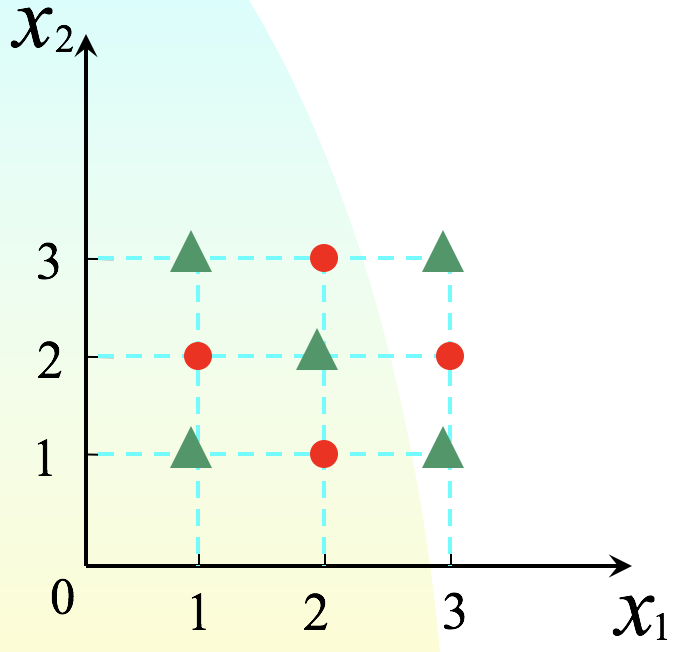
\includegraphics[width=0.35\linewidth]{img//fig0.png}
	\caption{两类数据分类要求}
\end{figure}\\[-0.5cm]
\subsection*{Analysis and Result}

\hs 首先我们观察到这两类数据在2维平面内是不存在线性的分类器,对于非线性的分类器,可以从2D、3D或者更加高维的超空间内进行分类。\\


{\kaishu{\large 2D分类 }}

\hs 在2D空间内,我们可以使用两对双曲线来实现,具体分类结果如图2所示:
\begin{figure}[htbp]
	\centering
	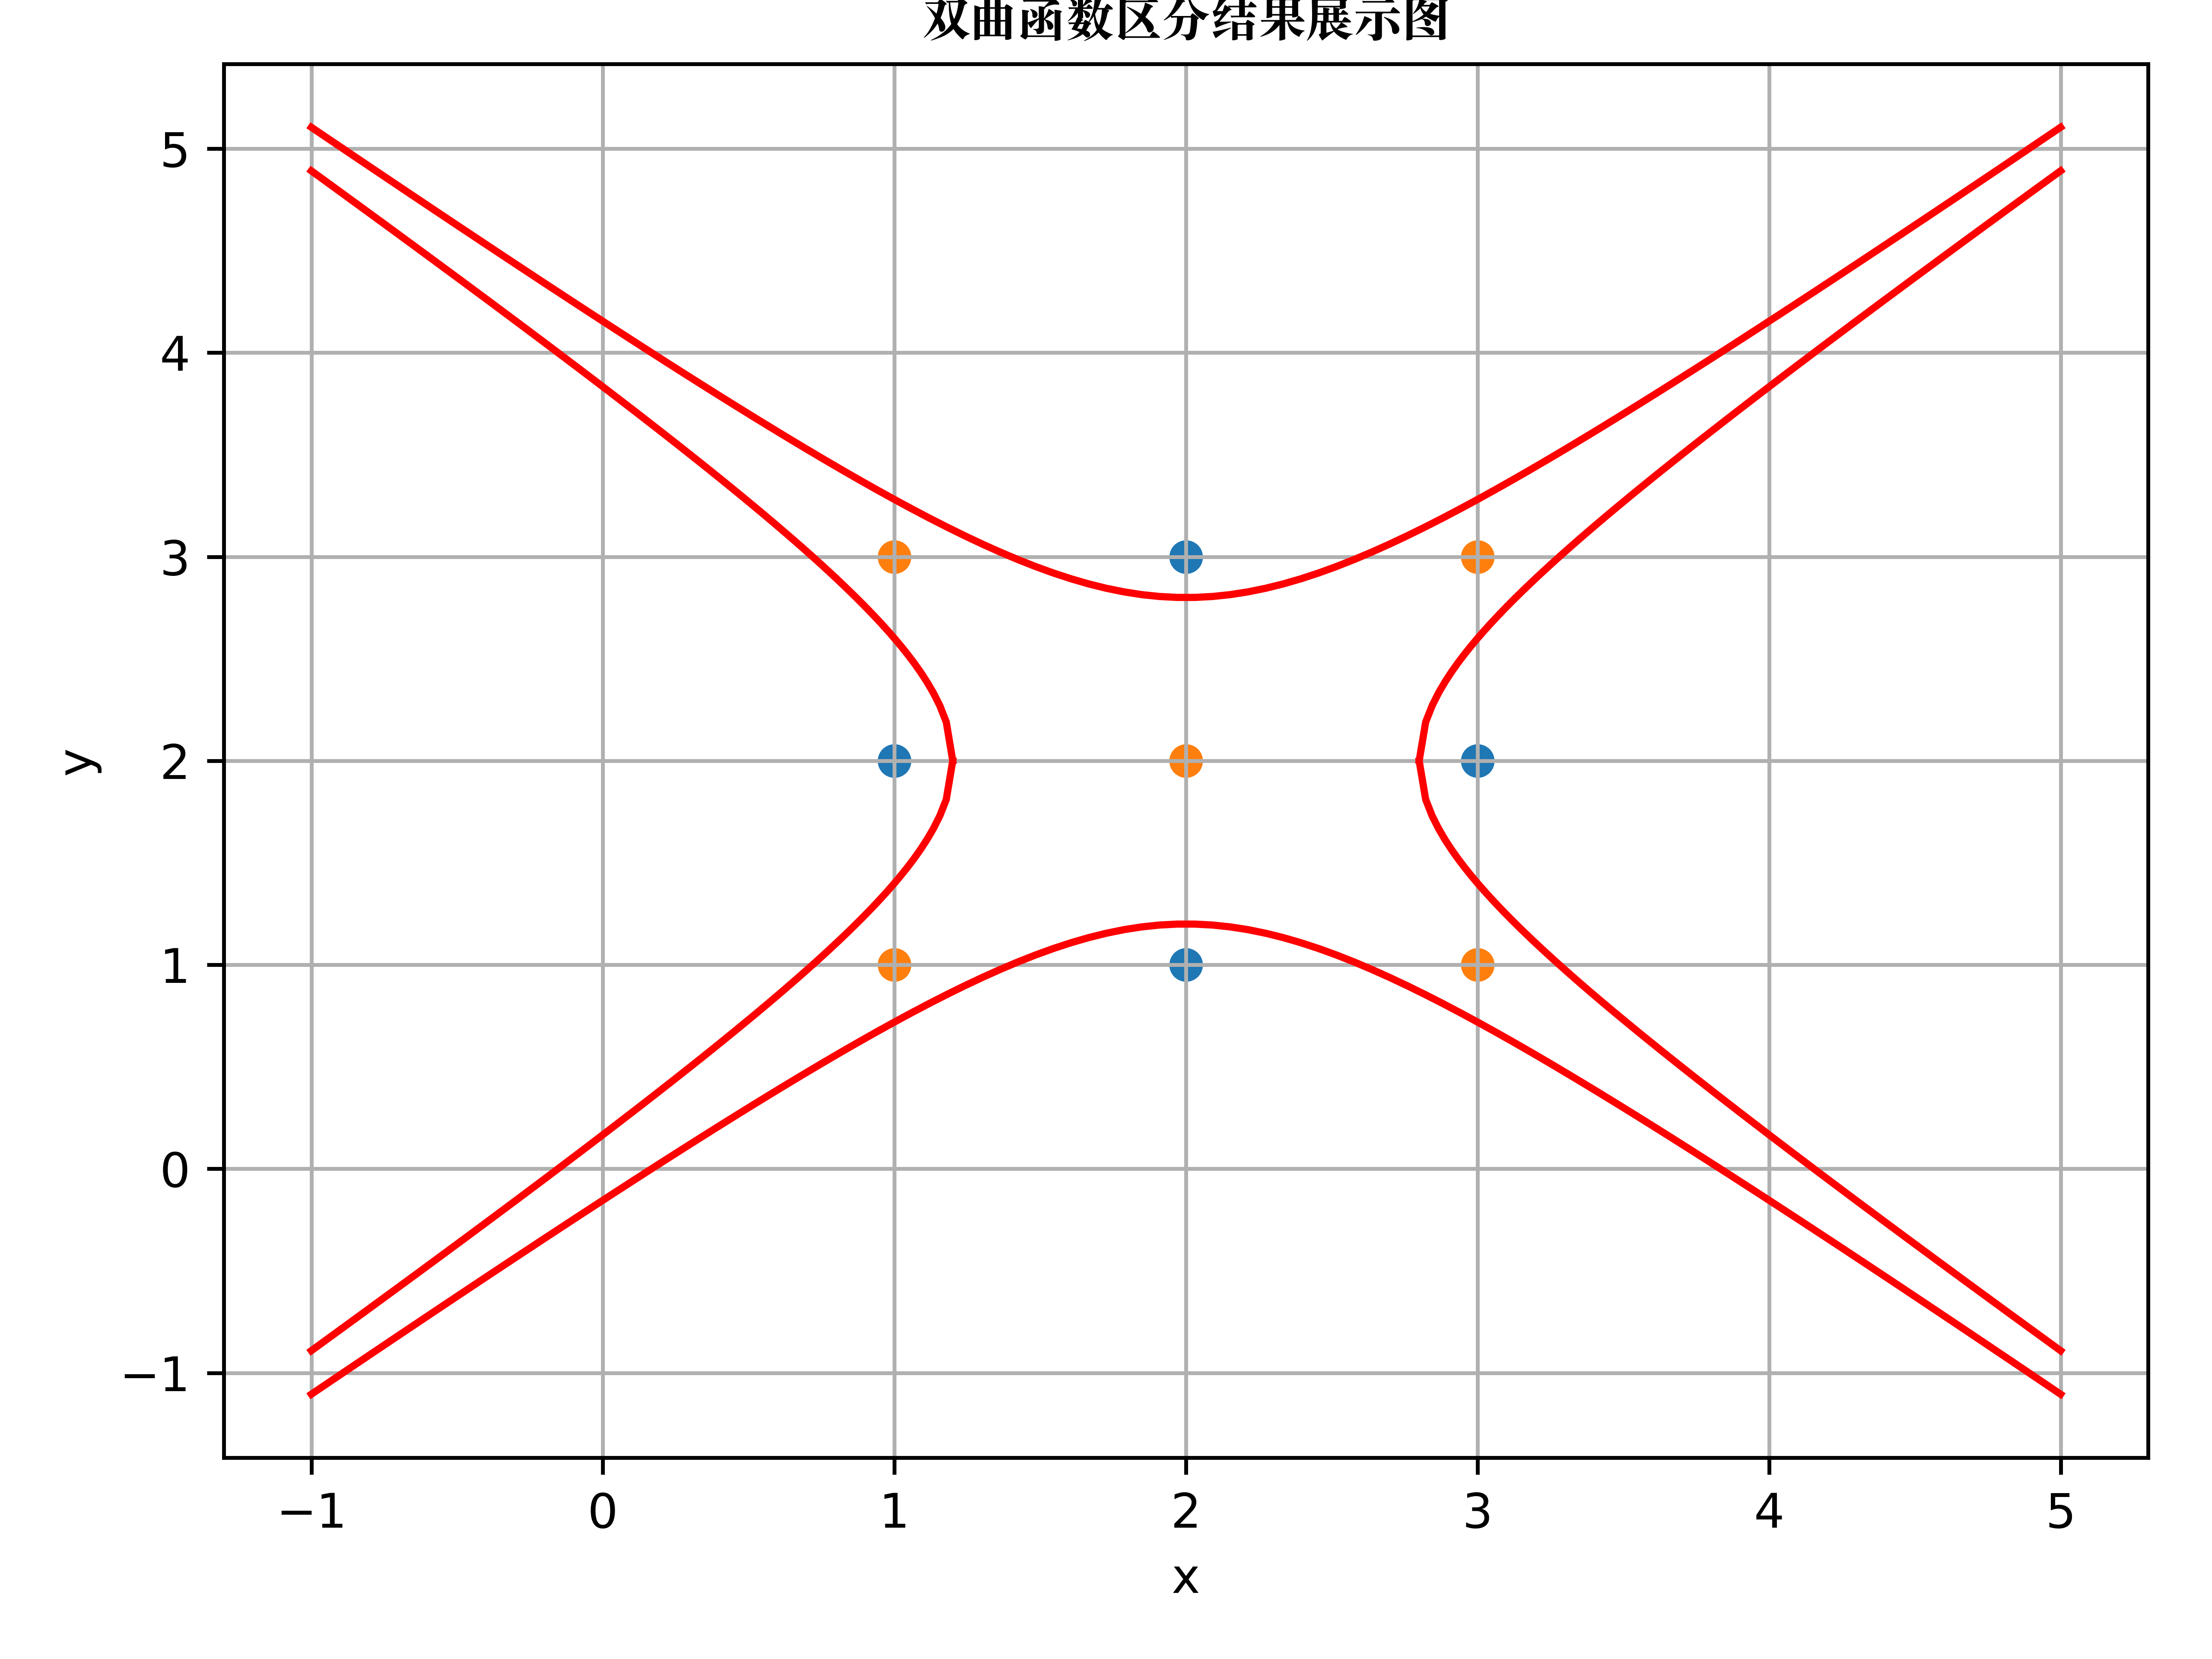
\includegraphics[width=0.45\linewidth]{img//fig2.png}
	\caption{两对双曲线分类结果}
\end{figure}

上述分类函数是根据$y=\frac{0.64}{x}$,平移(2,2),再旋转逆时针45$^\circ$得到,利用旋转的特性$u=\frac{x+y}{2},v=\frac{x-y}{2}$,代入即可得到最终分类界面曲线为:
\begin{equation*}
\left\lbrace \begin{array}{cc}
y = \sqrt{(x-2)^2+0.64}+2 & \text{上侧函数} \\
y = -\sqrt{(x-2)^2+0.64}-2 & \text{下侧函数}\\
x = \sqrt{(y-2)^2+0.64}+2 & \text{右侧函数} \\
x = -\sqrt{(y-2)^2+0.64}+2 & \text{左侧函数}
\end{array}\right. 
\end{equation*}\\

{\kaishu{\large 3D分类 }}

\hs 在3D空间内可以考虑$\sin(xy)$函数形式和立体圆环形式:

\hs 假设在3D空间内,数据点的z坐标都为零,这里可以利用$\sin(xy)$类函数对这两类数据进行分类,一类在$\sin(xy)$类函数上侧,一类为下侧。这里展示$\cos(xy)$的3D分界面:
\begin{figure}[htbp]
	\centering
	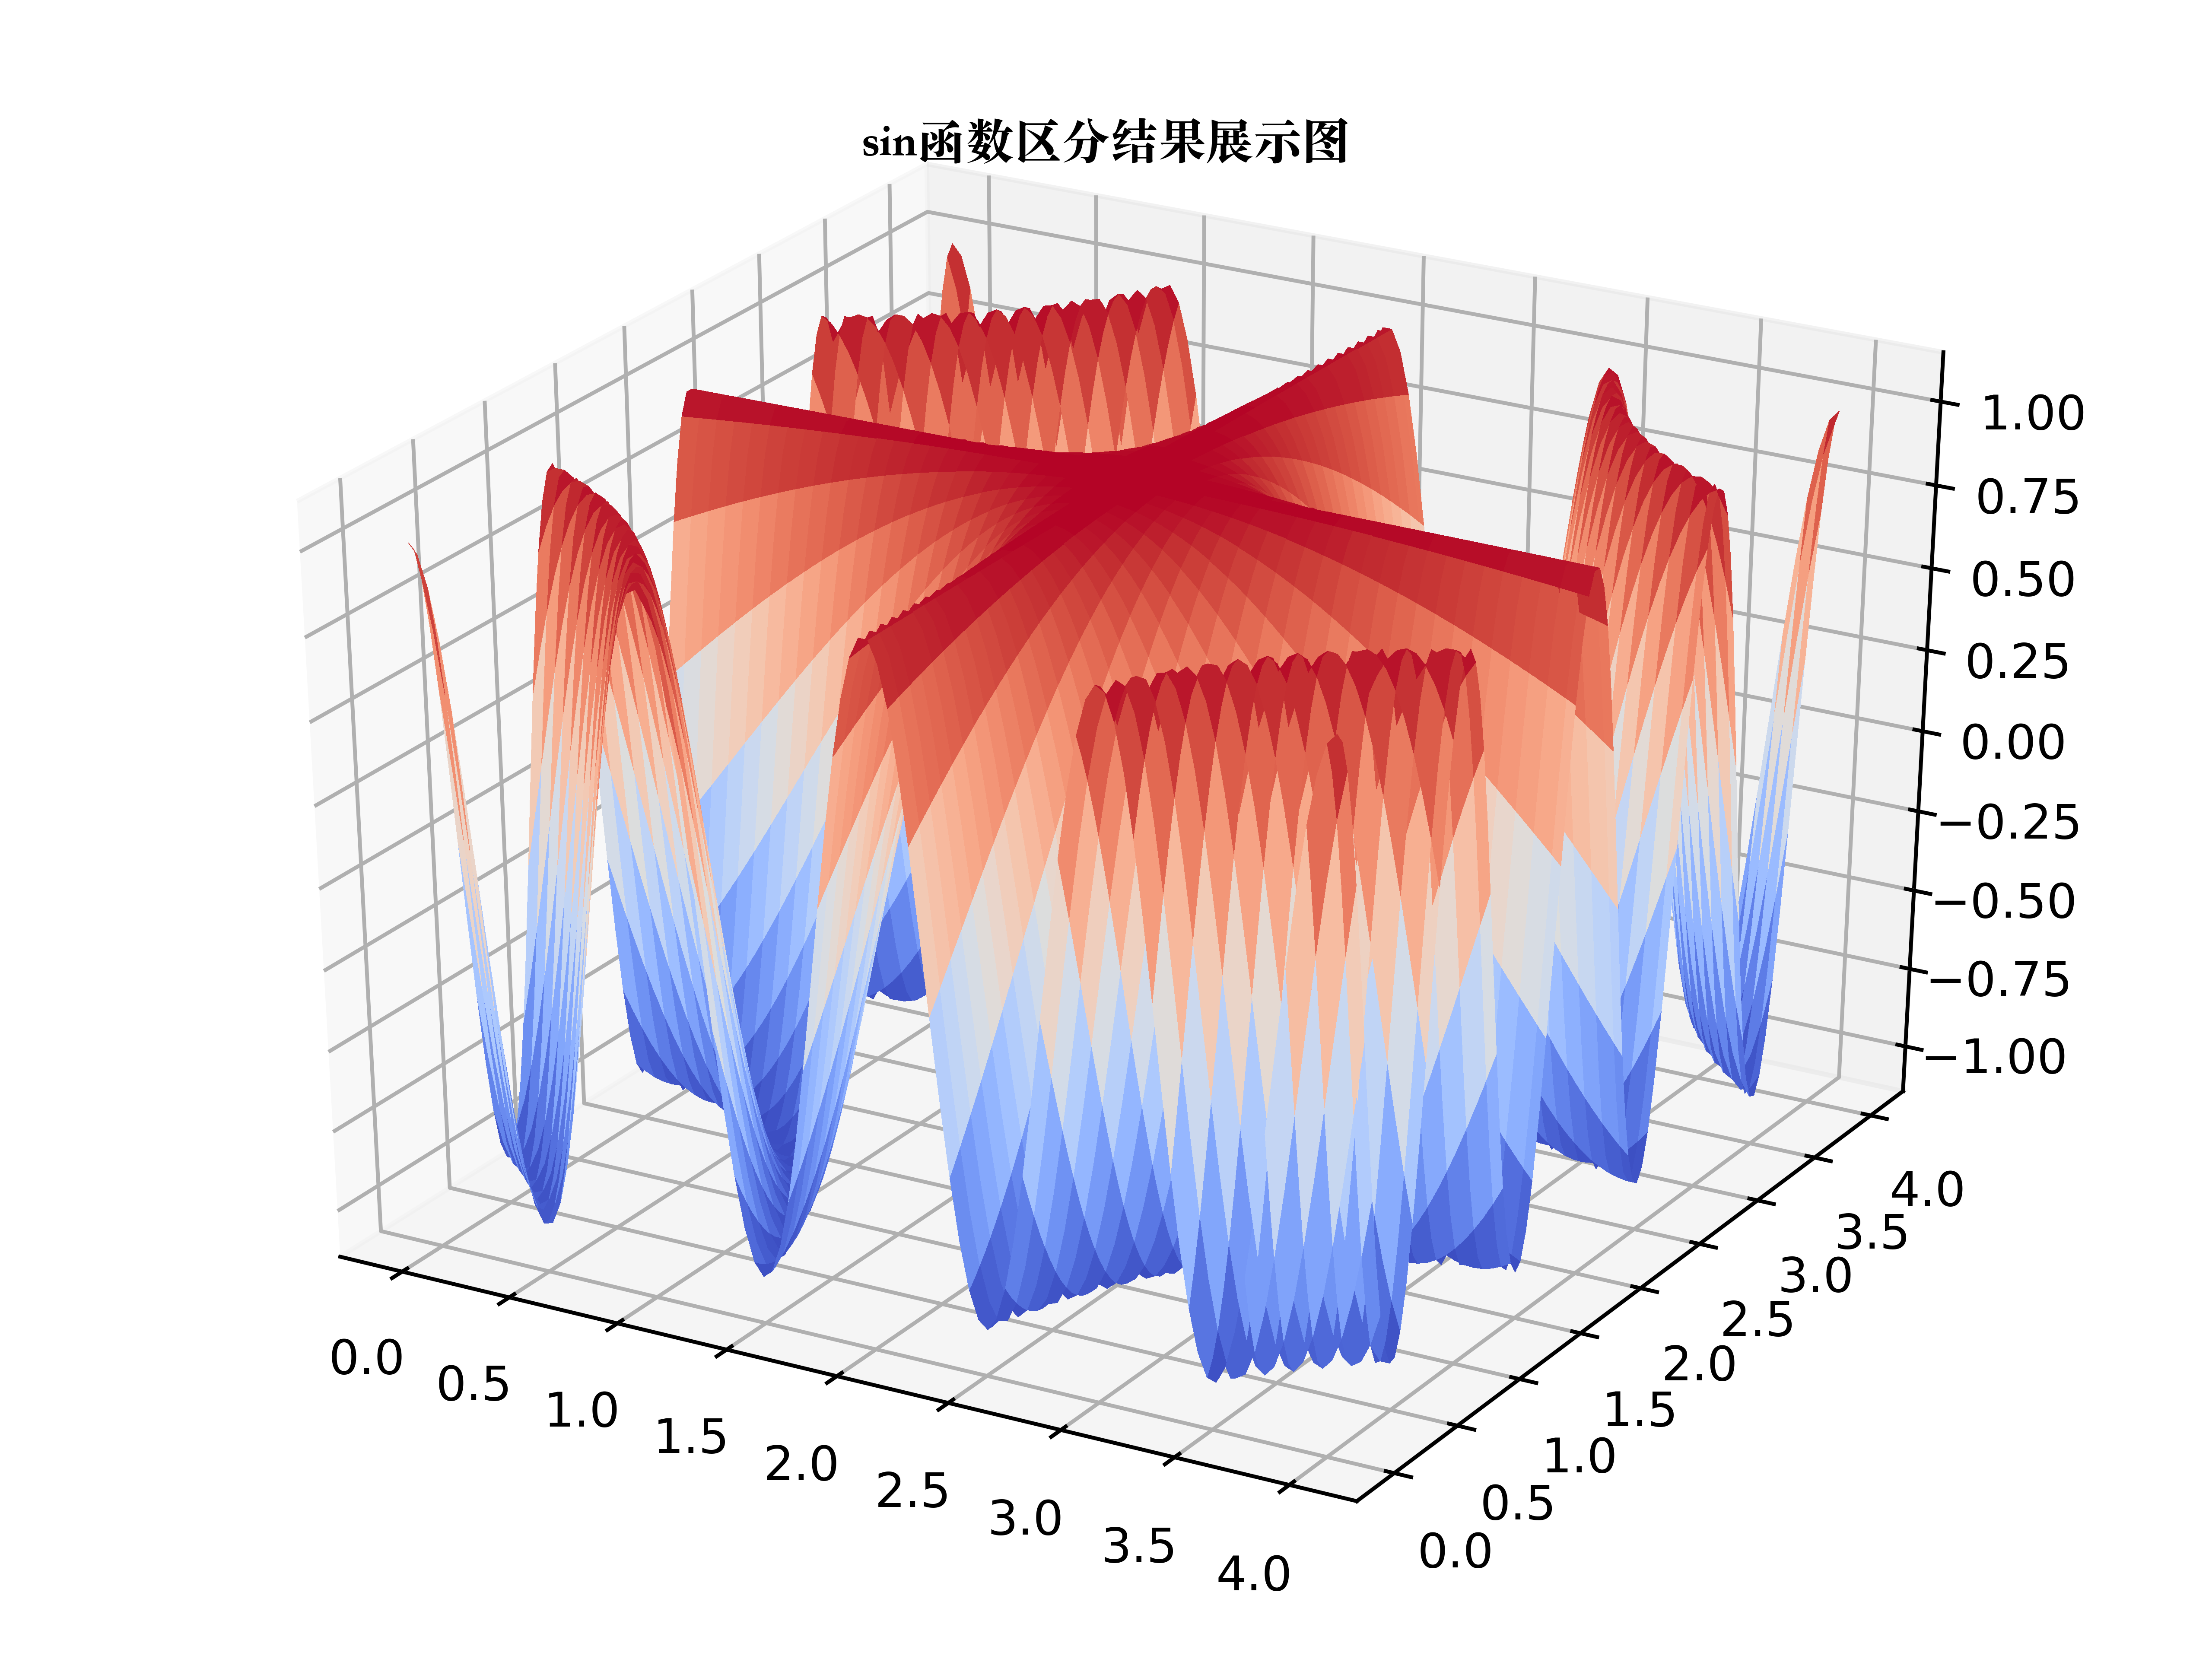
\includegraphics[width=0.5\linewidth]{img//fig3.png}
	\caption{$\sin$3D分类结果}
\end{figure}

再利用上述中平移和旋转的步骤,得到最终的分界面的函数形式如下:
\begin{equation*}
z = \sin(\pi (\frac{x+y}{2}-2)(\frac{x-y}{2}-2))=\sin(\pi\frac{x^2-y^2-8y+16}{4})
\end{equation*}

将上述两类数据坐标点代入到方程中,可以得到,红点值为$-\frac{\sqrt{2}}{2}$,绿色三角形点的值为1,因此红点都在分界面的上方($-\frac{\sqrt{2}}{2}$<0),而绿色三角形点都在分界面的下方(0<1),从而区分出两类数据。\\

\hs 此外在3D空间中可以利用立体的圆环通道来实现分类, 其立体圆环通道如下:
\begin{figure}[H]
	\centering
	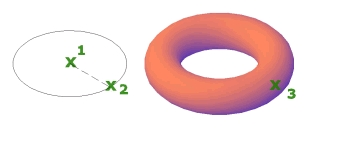
\includegraphics[width=0.5\linewidth]{img//fig4.jpg}
	\caption{3D圆环}
\end{figure}

在$x-z$平面内,立体圆环的截图是一个圆,其方程为:$(x-1)^2+z^2=0.2^2$。利用绕$z$轴旋转生成立体图像的性质,即$x$用$\sqrt{x^2+y^2}$代入,得到最后的方程如下:
\begin{equation*}
(\sqrt{x^2+y^2}-1)^2+z^2=0.2^2
\end{equation*}

为了方便观察将其投影到$x-y$平面,结果如下:
\begin{figure}[htbp]
	\centering
	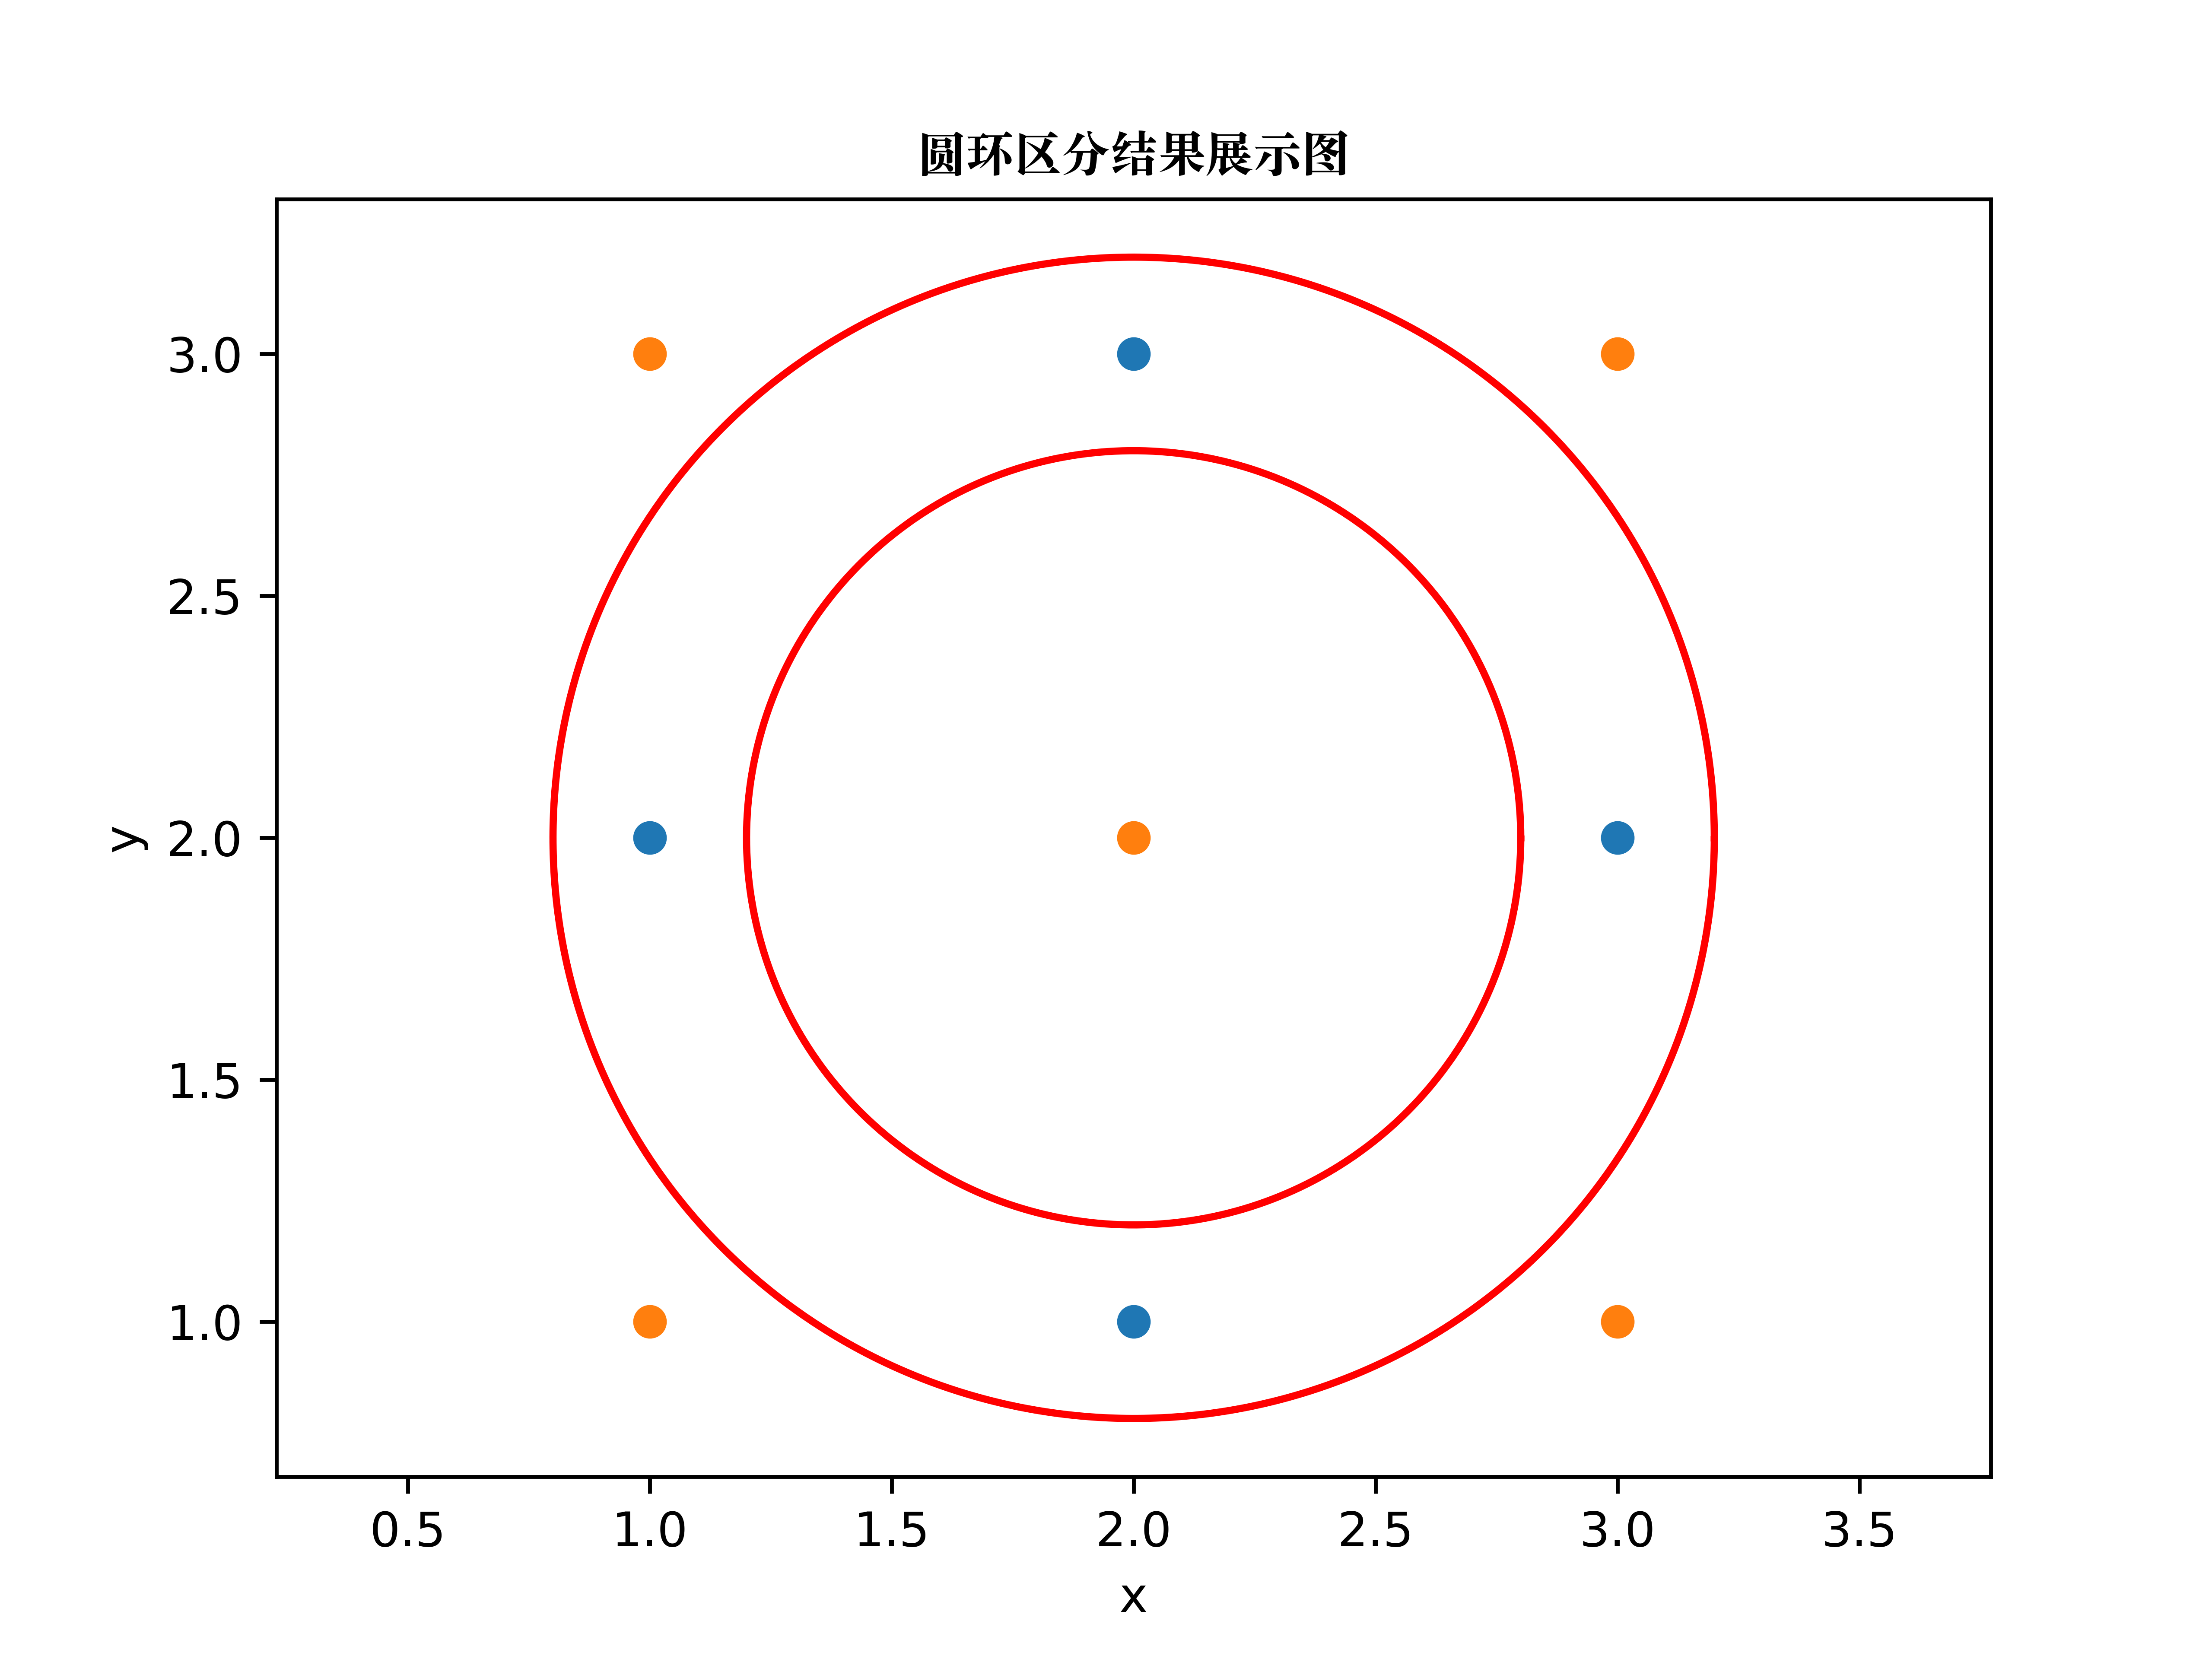
\includegraphics[width=0.5\linewidth]{img//fig5.png}
	\caption{3D圆环在$x-y$平面内的结果}
\end{figure}

在圆环内为一类,在圆环外另一类。  

\section{Problem Two}
{\kaishu{\large 迭代修正求权向量}}

\begin{equation*}
\begin{split}
\omega_1 &= \{(1,1); (2,0); (2,1); (0,2); (1,3) \}\\
\omega_2 &= \{(-1,2); (0,0); (-1,0); (-1,-1); (0,-2))\}
\end{split}
\end{equation*}
求解如下问题:
\begin{itemize}	
	\item 迭代修正求权向量的方法,求上述两类的线性识别函数
	\item 迭代修正求权向量的方法,求上述两类的线性识别界面
	\item 画出该识别界面将训练样本的区分结果图示 
\end{itemize}


\subsection*{Analysis and Result}

{\kaishu{\large $S$ 集合生成}}

\hs 权空间将识别界面问题转为求解权向量$w$的问题,在利用其求解两类分类问题时,可以利用小技巧将识别界面约束条件全部转换为$>0$的形式,即:
\begin{equation*}
 \left\lbrace \begin{array}{c}
 w^Tx_i '>0 \\
 w^Ty_i '<0
 \end{array} \right.  \Longrightarrow 
  \left\lbrace \begin{array}{c}
 w^Tx_i '>0 \\
 w^T(-y_i ')>0
 \end{array} \right.
\end{equation*}

再令$S=\{x_1',x_2',\dots,-y_1',-y_2'\dots\}=\{z_1',z_2',\dots\}$,即可得:$w^Tz_i '>0$ 

{\kaishu{\large 线性识别函数}}

\hs 根据线性识别函数的定义,我们可以得到:
\begin{equation*}
D(x_i')=w^Tx_i'>0, ~D(y_i')=w^Ty_i'<0
\end{equation*}


{\kaishu{\large 线性识别界面}}


\hs 根据迭代法的步骤,最后求解出的线性界面为:
\begin{equation*}
4w_1+2w_2-1=0
\end{equation*}
       
{\kaishu{\large 识别界面区分结果}}       

\hs 图6为线性界面区分两类数据结果:

\begin{figure}[htbp]
	\centering
	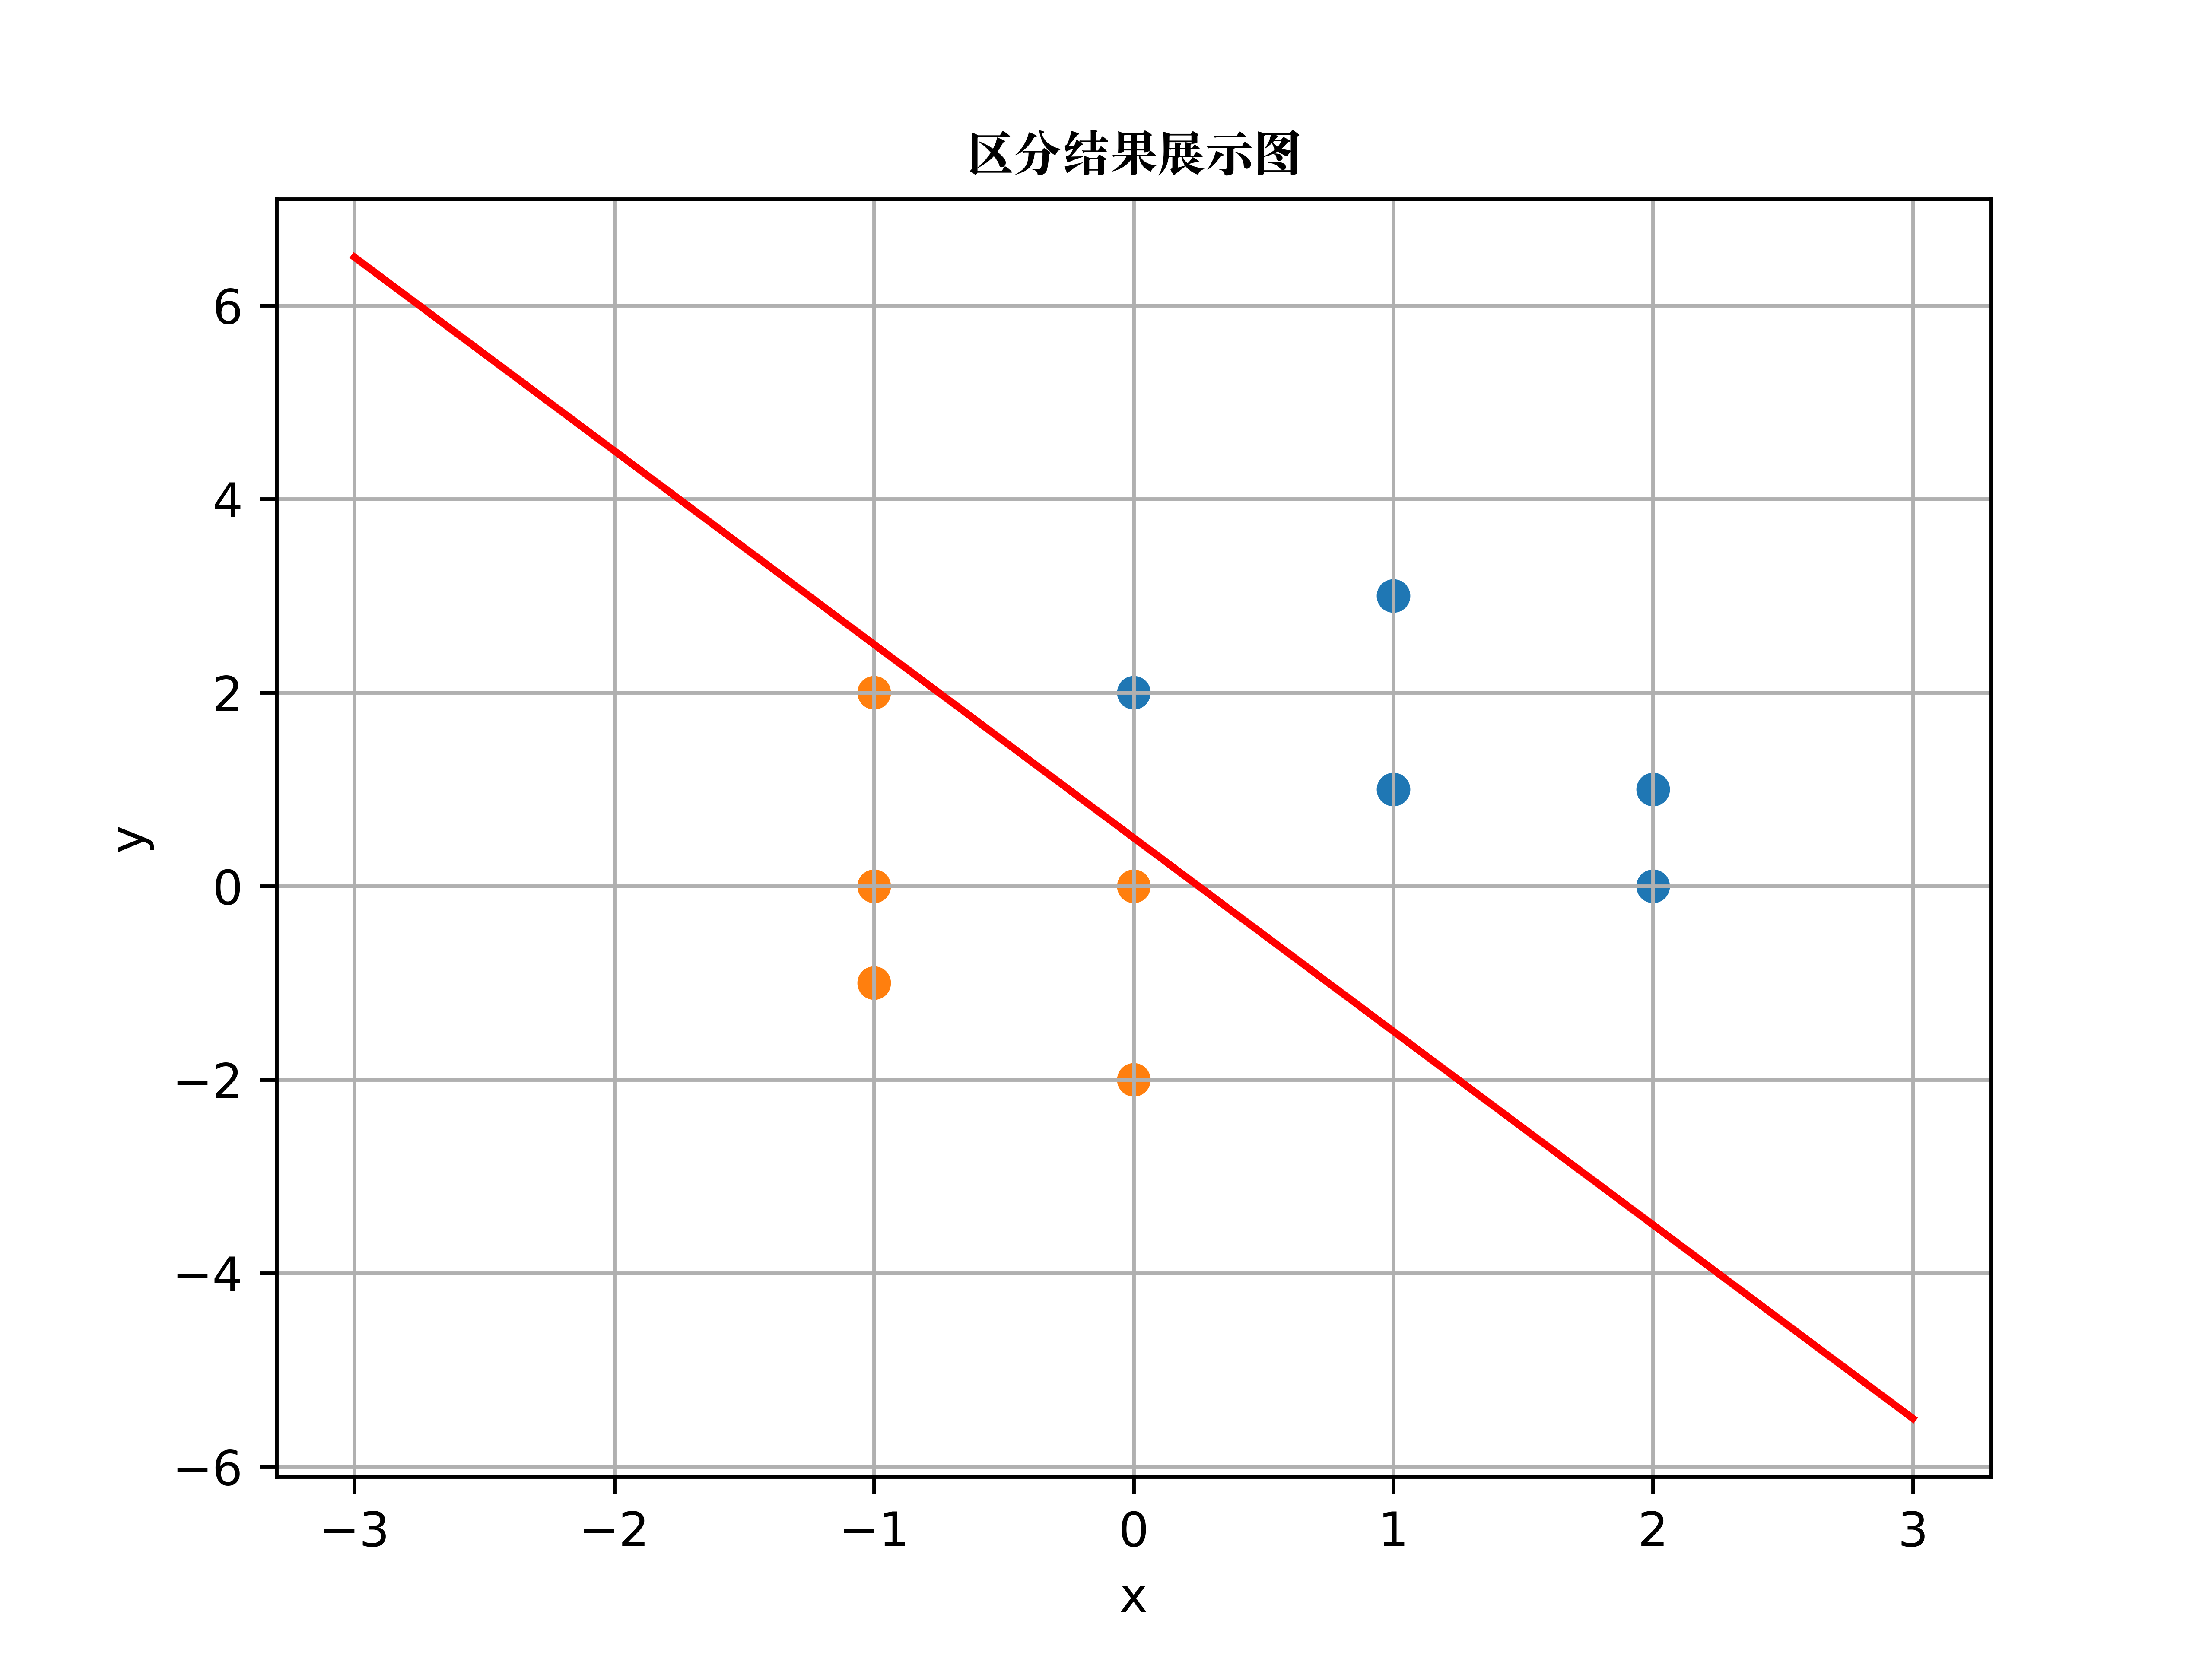
\includegraphics[width=0.5\linewidth]{img//fig1.png}
	\caption{迭代修正权空间区分结果}
\end{figure}

{\kaishu{\large 分析思考}}

\hs 经过测试迭代修正求权向量法对初值比较敏感,比如上面结果结果中,我选取的初始的$w=\{0,0,-3\}$,但将这个参数改为$w=\{0,0,0\}$时,得到的界面结果就不一样了,区分界面方程如下:
\begin{equation*}
4w_1+w_2-1=0
\end{equation*}

区分界面结果如下图7:
   
   \begin{figure}[htbp]
   	\centering
   	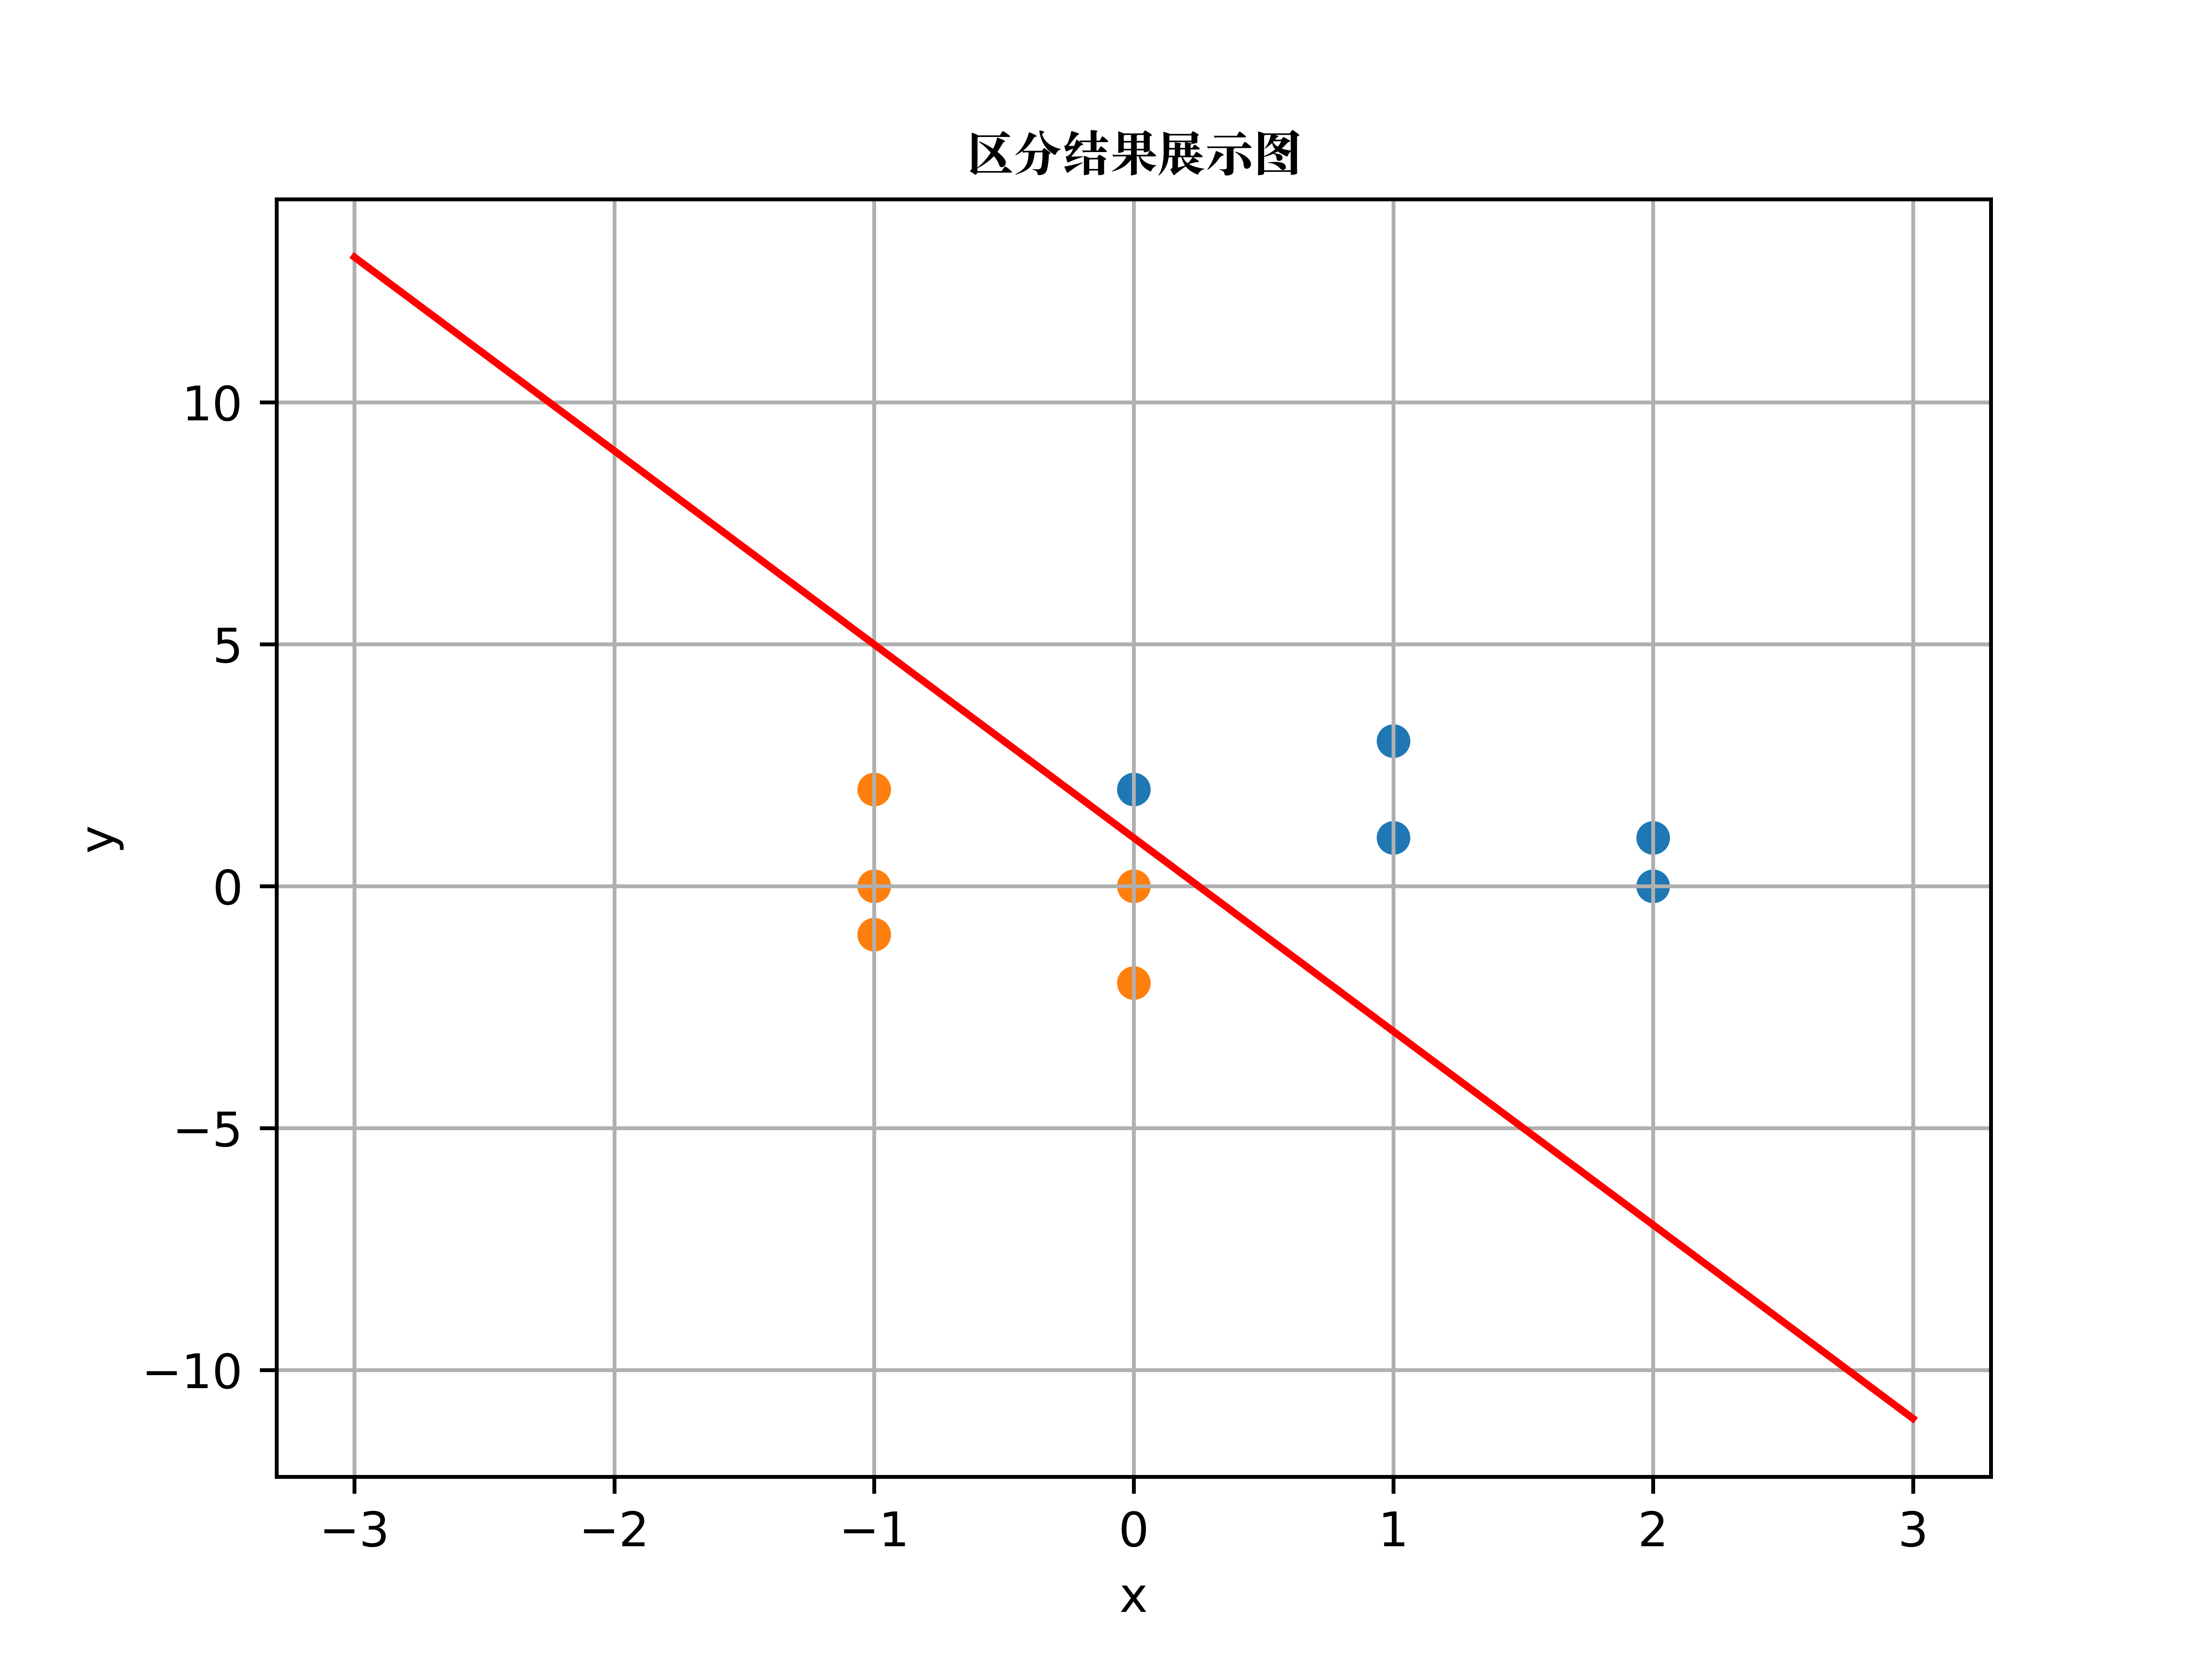
\includegraphics[width=0.5\linewidth]{img//fig6.png}
   	\caption{初始权重为$w=\{0,0,0\}$迭代修正权空间区分结果}
   \end{figure}
    
  \hs 并且迭代修正的权向量法对这些界面方程的“打分”都是一样的,也就是说只要分类结果是对的,此类算法认为这些界面的“打分”都是一致的,这一点不像SVM,SVM是最小化“风险”,它会选取“风险”最小的风界面,这些所有正确分类分界面的“打分”是不一致的。
  
  \hs 当然对于迭代参数$c$来说,其值结果只会成倍的方法$w_1,w_2,w_3$, 而成倍方法并不会影响最后的界面方程。\\
  
  
  {\kaishu{\large 改进迭代修正权向量法}}
  
  \hs 上述算法的计算时间偏长,因为其算法每改变$w_k$需要对整个样本都进行遍历,注意这个改变只是针对$w^Tz_i '>0$ 的一个样本而已,并没有利用后面样本的信息,因此这样的计算代价是比较高的。改进的迭代修正的权向量法,将在$S$的全体样本中,挑选出不满足条件$w^Tz_i '>0$ 的样本,求其平均值$Z'$,再利用均值进行修正。
  
  \hs 初始化权重为$w=\{0,0,0\}$,得到的界面方程如下:
   \begin{equation*}
  2.4w_1+1.3w_2-1=0
  \end{equation*}
  
 \hs 改进算法界面分类结果如下图8:
    \begin{figure}[H]
 	\centering
 	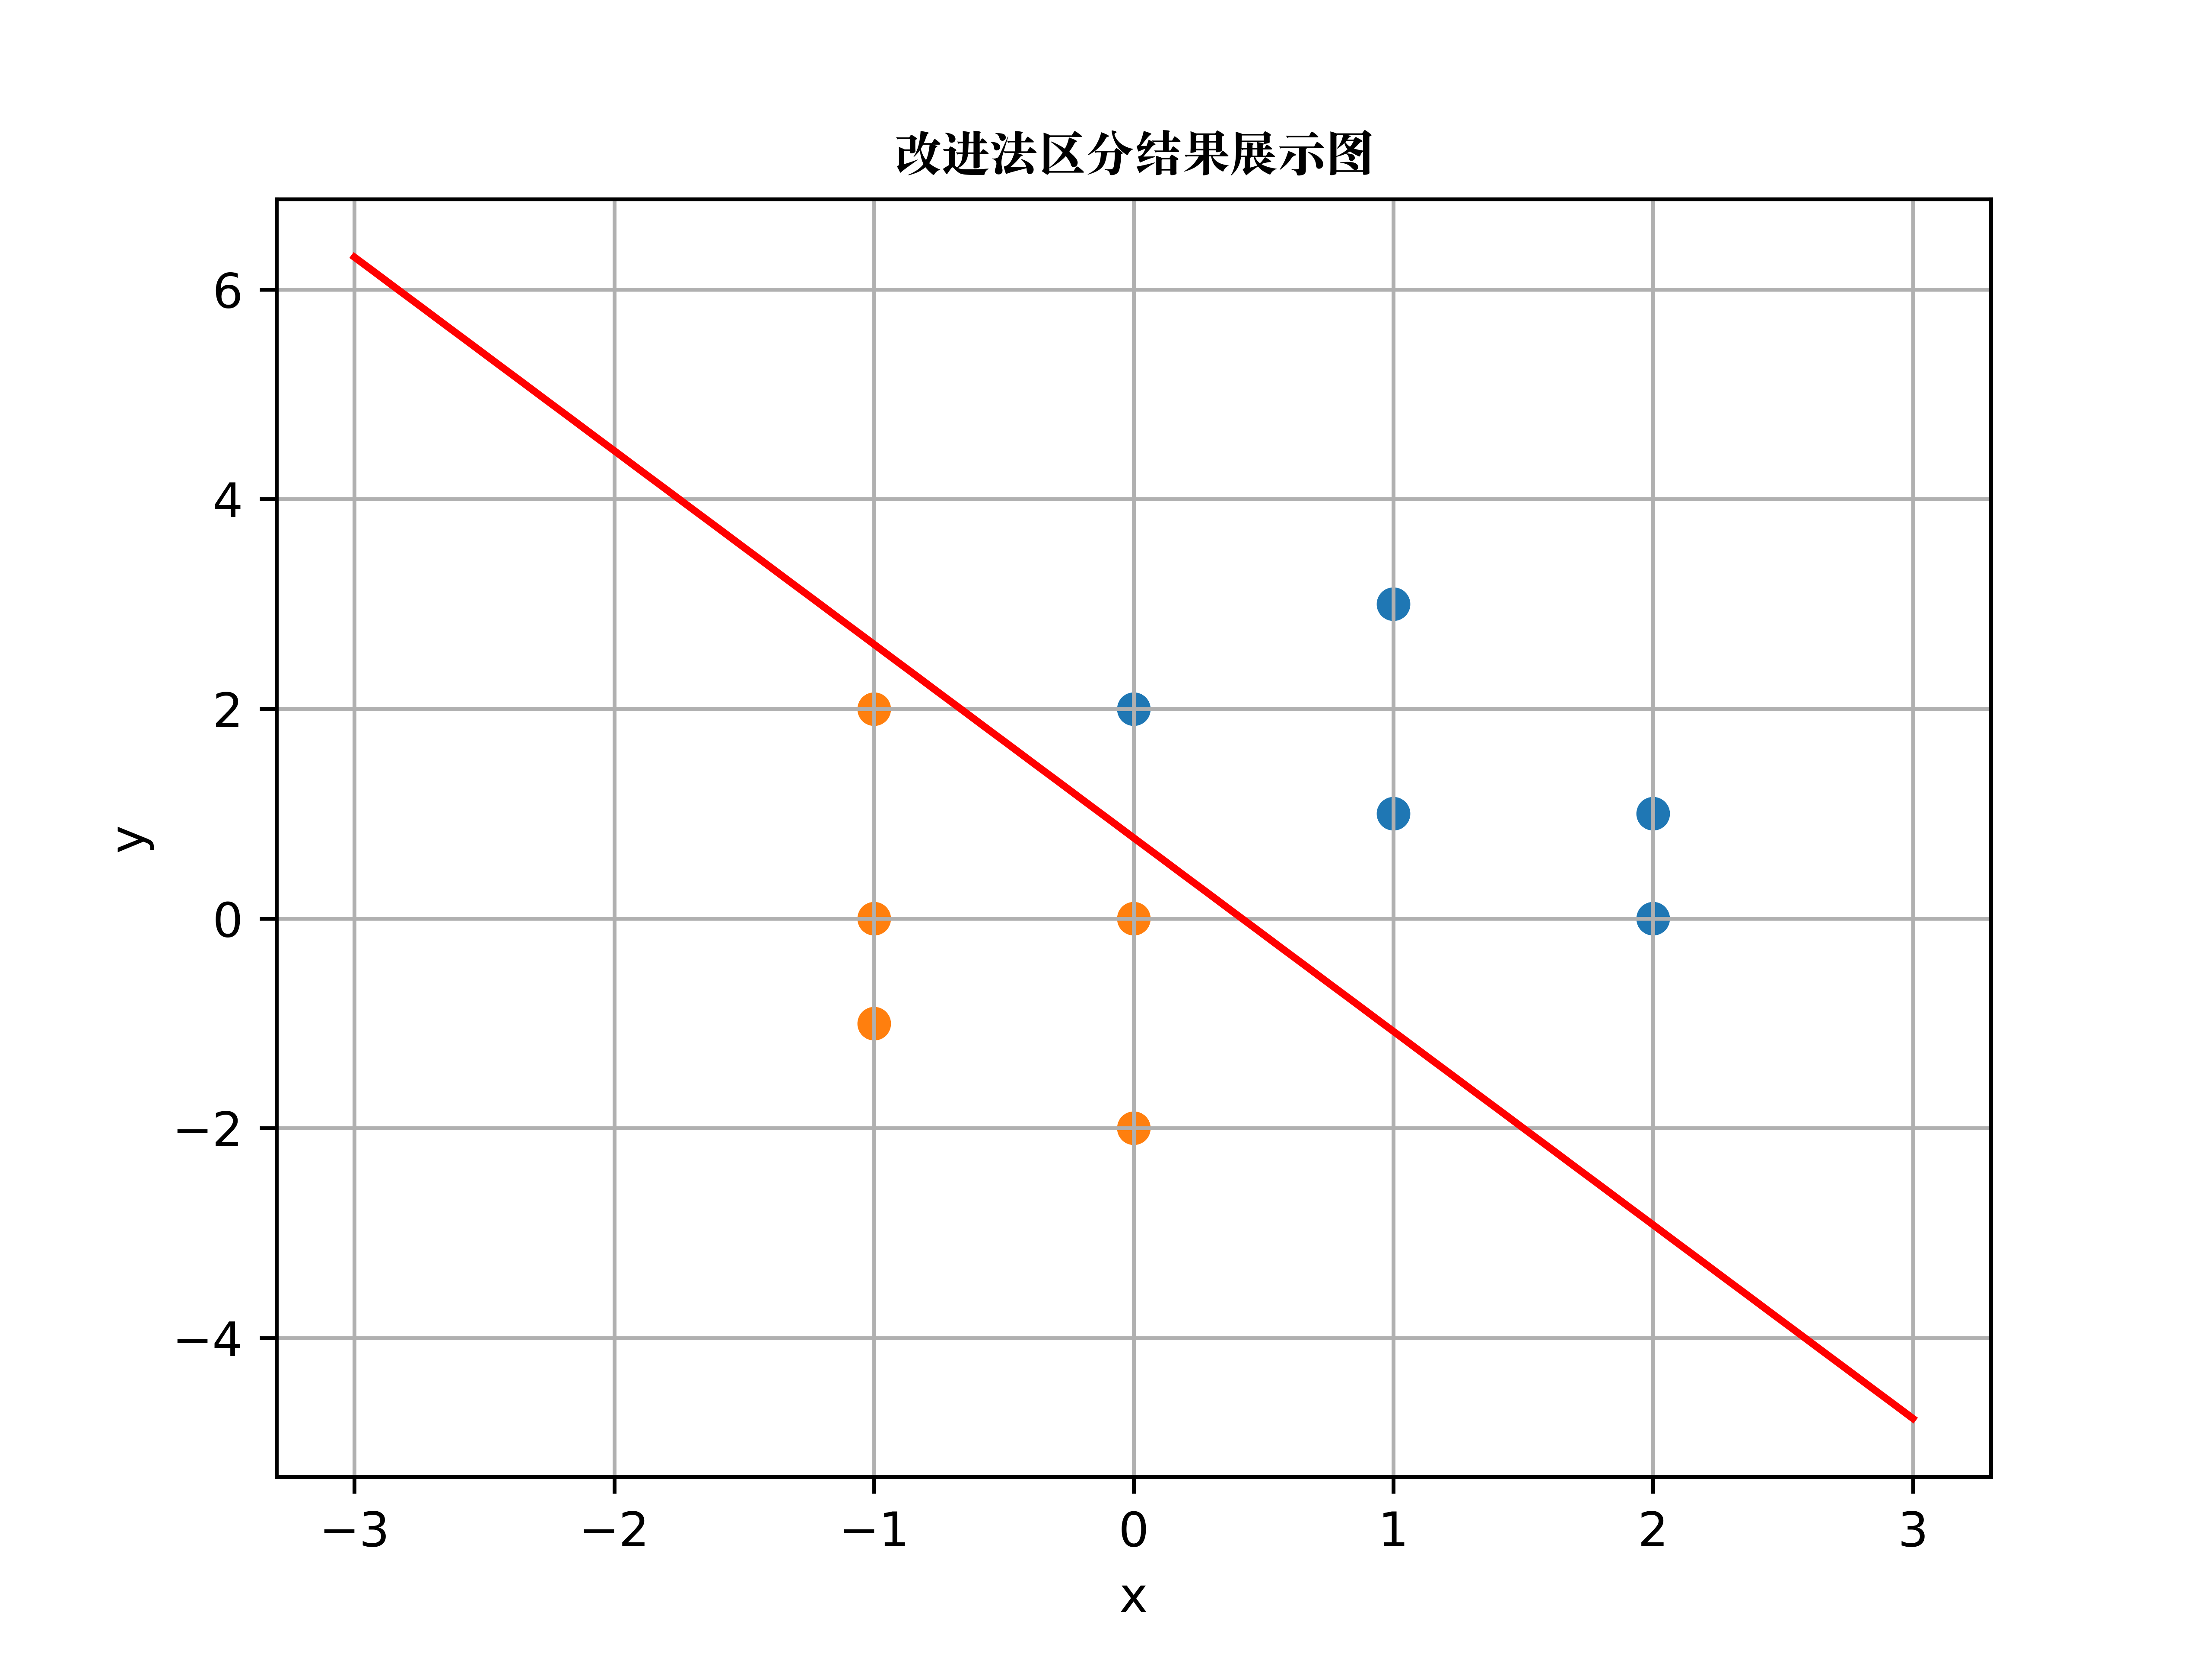
\includegraphics[width=0.5\linewidth]{img//fig7.png}
 	\caption{初始权重为$w=\{0,0,0\}$改进迭代修正权空间区分结果}
 \end{figure}
  
  
  \hs 我统计一下两种算法的$w$向量的迭代次数以及一共进行的点击操作次数(两者一定程度能反应收敛的速度),结果如下图9:
    \begin{figure}[H]
  	\centering
  	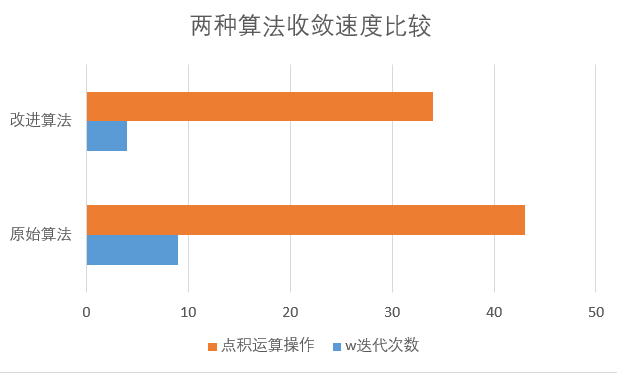
\includegraphics[width=0.5\linewidth]{img//fig8.png}
  	\caption{两种算法迭代收敛速度比较}
  \end{figure}
  
  上述图9显示,无论是$w$的迭代次数还是点击操作次数改进的算法都优于原始算法,此外对两种算法的运行时间进行统计,原始算法运行时间为0.000932s,改进算法的运行时间为0.000847s(平台为:MacBook Pro,Intel Core i5,3.1GHz,内存8 GB),说明了在利用了全部样本的信息之后,算法的收敛速度得到了增强。
\end{document}
